\documentclass{beamer}

\usepackage{graphicx}
\usepackage{tikz}
\usetikzlibrary{shapes.callouts}
\usepackage{multirow}

%\usetheme{AnnArbor}
%\usetheme{Antibes}
%\usetheme{Bergen}
%\usetheme{Berkeley}
%\usetheme{Berlin}
%\usetheme{Boadilla}
%\usetheme{boxes}
%\usetheme{CambridgeUS}
%\usetheme{Copenhagen}
%\usetheme{Darmstadt}
%\usetheme{default}
%\usetheme{Frankfurt}
%\usetheme{Goettingen}
%\usetheme{Hannover}
%\usetheme{Ilmenau}
%\usetheme{JuanLesPins}
%\usetheme{Luebeck}
%\usetheme{Madrid}
%\usetheme{Malmoe}
%\usetheme{Marburg}
%\usetheme{Montpellier}
%\usetheme{PaloAlto}
%\usetheme{Pittsburgh}
%\usetheme{Rochester}
%\usetheme{Singapore}
%\usetheme{Szeged}
%\usetheme{Warsaw}

\title[EAE105A]{EAE105A \\ Introducci\'on a la Econom\'ia}

\subtitle[Teor\'ia de la Inflaci\'on]{Teor\'ia de la Inflaci\'on}

\institute[PUC]{Instituto de Econom\'ia\\
Pontificia Universidad Cat\'olica de Chile}

\date[$\:$]

\subject{Teor\'ia de la Inflaci\'on}

\AtBeginSection[]{
\begin{frame}<beamer>{Contenidos}
\tableofcontents[currentsection, currentsubsection]
\end{frame}}

\begin{document}
\maketitle

\begin{frame}
\frametitle{Introducci\'on}
\begin{itemize}
\setlength\itemsep{1.4em}
\item En secciones anteriores hemos visto c\'omo medir la \textbf{inflaci\'on}.\\
\begin{itemize}
\setlength\itemsep{1.0em}
\item[-] Cambio porcentual en el IPC.
\item[-] Cambio porcentual en el deflactor del PIB.
\item[-] Cambio porcentual en el IPP.
\end{itemize}
\item Existen marcadas diferencias \textbf{inter} e \textbf{intra} paises del nivel de inflaci\'on.\\
\begin{itemize}
\setlength\itemsep{1.0em}
\item[-] Algunos paises enfrentan hiperinflaciones otros deflaciones.
\item[-] El nivel de inflaci\'on de un pa\'is puede cambiar significativamente en el tiempo.
\end{itemize}
\end{itemize}
\end{frame}

%\begin{frame}
%\frametitle{Introducci\'on}
%\begin{itemize}
%\item Es importante adem\'as notar que la inflaci\'on es una preocupaci\'on real de las personas.
%\end{itemize}
%\begin{center}
%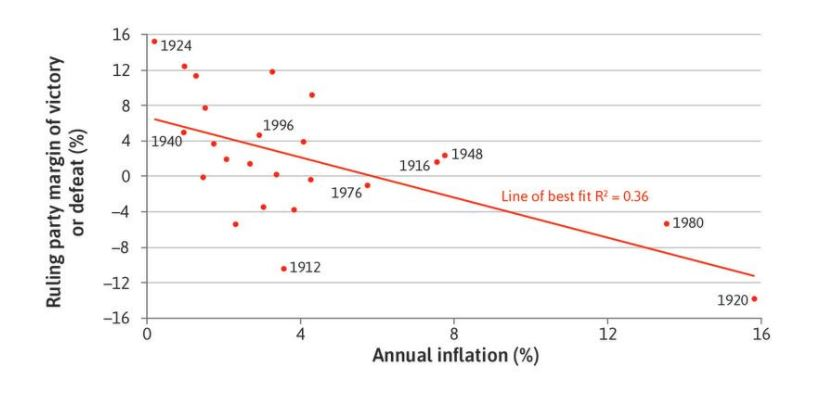
\includegraphics[scale=0.455]{Figuras/Margin}
%\end{center}
%\end{frame}

\begin{frame}
\frametitle{Introducci\'on}
\begin{itemize}
\setlength\itemsep{1.4em}
\item Algunas preguntas interesantes:\\
\begin{itemize}
\setlength\itemsep{1.0em}
\item[-] ?`Qu\'e cosas determinan que un pa\'is enfrente inflaci\'on?
\item[-] ?`Qu\'e factores determinan la magnitud de la inflaci\'on?
\item[-] ?`Qu\'e costos supone la inflaci\'on para la poblaci\'on?
\end{itemize}
\item Estudiaremos un modelo simple que permite estudiar las preguntas anteriores.
\item En lo que sigue se presenta la \textbf{Teor\'ia cl\'asica de la inflaci\'on}.
\end{itemize}
\end{frame}

\begin{frame}
\frametitle{El valor del dinero}
\begin{itemize}
\setlength\itemsep{1.4em}
\item Resulta \'util considerar \textbf{dos interpretaciones} alternativas del nivel de precios:\\
\begin{itemize}
\setlength\itemsep{0.7em}
\item[-] Precios de los bienes y servicios en la econom\'ia.
\item[-] Valor o Precio del dinero.
\end{itemize}
\item Si el valor de una canasta es $P$ unidades de dinero, el valor de una unidad de dinero es $\frac{1}{P}$ de canasta.
%\item Notar que la interpretaci\'on \'ultima otorga la naturaleza de \textbf{bien com\'un} al dinero. ?`Qu\'e rige su precio?
\end{itemize}
\end{frame}

\begin{frame}
\frametitle{Interacci\'on oferta y demanda de dinero}
\begin{itemize}
\setlength\itemsep{1.4em}
\item La interacci\'on entre la oferta por dinero y la demanda por dinero determina el precio del mismo.
\item Debe notarse que los mecanismos no son distintos a los estudiados en otros bienes.\\
\begin{itemize}
\setlength\itemsep{0.8em}
\item[-] Exceso de demanda, empuja el precio hacia arriba.
\item[-] Exceso de oferta, empuja el precio hacia abajo.
\end{itemize}
\item Necesitamos entender los \textbf{determinantes de la oferta y la demanda por dinero}.
\end{itemize}
\end{frame}

\begin{frame}
\frametitle{Oferta de dinero}
\begin{itemize}
\setlength\itemsep{1.4em}
\item \textbf{Dinero:} Medio de cambio utilizado para la compra de bienes y servicios.
\item En general el banco central es el encargado de la oferta de dinero.
\item Los bancos comerciales, mediante sus actividades de pr\'estamos, tambi\'en son capaces de afectar la oferta de dinero.
\end{itemize}
\end{frame}

\begin{frame}
\frametitle{Demanda de dinero}
\begin{itemize}
\setlength\itemsep{1.4em}
\item La demanda por dinero refleja el deseo de las personas de mantener riqueza en forma \textbf{l\'iquida}.
\item Muchos factores determinan la demanda por dinero:\\
\begin{itemize}
\setlength\itemsep{0.6em}
\item[-] Facilidad de conversi\'on entre dinero y otros medios de atesorar riqueza.
\item[-] Existencia de medios de pago alternativos: e.g. Tarjetas de cr\'edito.
\item[-] Tasa de inter\'es de otros activos.
\end{itemize}
\item Un determinante resalta entre los dema\'as. El \textbf{nivel de precios}.
\end{itemize}
\end{frame}

\begin{frame}
\frametitle{Demanda de dinero}
\begin{itemize}
\setlength\itemsep{1.4em}
\item A diferencia de otros bienes, el dinero permite la compra y venta de otros bienes directamente.
\item La cantidad de dinero que se demanda depende del precio de dichos bienes.
\item La demanda por dinero es creciente:\\
\begin{itemize}
\setlength\itemsep{0.8em}
\item[-] Nivel de precios alto $\Rightarrow$ demanda por dinero alta.
\item[-] Nivel de precios bajo $\Rightarrow$ demanda por dinero baja.
\end{itemize}
\end{itemize}
\end{frame}

\begin{frame}
\frametitle{Interacci\'on oferta y demanda de dinero}
\begin{itemize}
\setlength\itemsep{1.4em}
\item ?`Qu\'e asegura que la oferta y la demanda por dinero se equilibren?
\item La respuesta depende del horizonte temporal que observemos.\\
\begin{itemize}
\setlength\itemsep{0.8em}
\item[-] \textbf{Largo Plazo:} El nivel de precios se equilibra.
\item[-] \textbf{Corto Plazo:} Otras variables llevan al equilibrio.
\end{itemize}
\item En esta secci\'on nos preocupamos por el equilibrio de largo plazo.
\end{itemize}
\end{frame}

\begin{frame}
\frametitle{Interacci\'on oferta y demanda de dinero}
\begin{center}
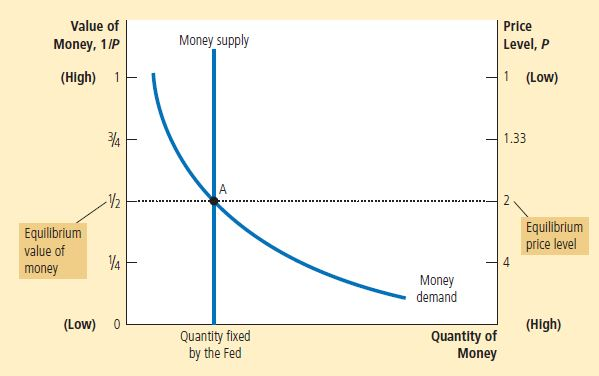
\includegraphics[scale=0.556]{Figuras/Equilibrio1}
\end{center}
\end{frame}

\begin{frame}
\frametitle{Intereacci\'on oferta y demanda por dinero (Ejemplo)}
\begin{itemize}
\setlength\itemsep{1.4em}
\item Pongamos a trabajar el instrumental aprendido. ?`Qu\'e implica un aumento de la oferta de dinero?
\item Lo anterior desplazar\'ia la curva de oferta de dinero a la derecha.\\
\begin{itemize}
\item[-] El valor del dinero que resultar\'ia de equilibrio ser\'ia menor al original.
\end{itemize}
\item La \textbf{Teor\'ia cl\'asica de la inflaci\'on} postula que mientras la demanda por dinero sea constante, la inflaci\'on es causada por la tasa de crecimiento de la oferta de dinero.
\end{itemize}
\end{frame}

\begin{frame}
\frametitle{Interacci\'on oferta y demanda de dinero (Ejemplo)}
\begin{center}
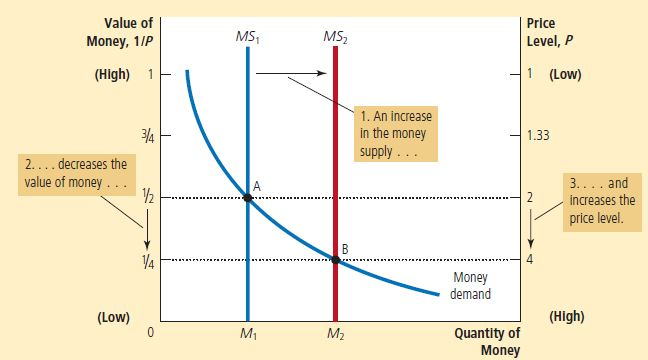
\includegraphics[scale=0.556]{Figuras/Equilibrio2}
\end{center}
\end{frame}

\begin{frame}
\frametitle{Interacci\'on oferta y demanda por dinero (Ejemplo)}
\begin{itemize}
\item ?`C\'omo resulta el proceso de ajuste?\\
\vspace{2mm}
\begin{itemize}
\setlength\itemsep{0.9em}
\item[1.] Las personas se encuentran con m\'as dinero dado el aumento de la oferta.
\item[2.] Las personas se deshacen del exceso de oferta mediante, compra de bienes y servicios y pr\'estamos.
\item[3.] El aumento por la demanda de bienes y servicios aumenta el precio de los bienes y servicios.
\item[4.] El aumento en los precios, aumenta la demanda por dinero.
\item[5.] El mercado monetario alcanza un nuevo equilibrio.
\end{itemize}
\end{itemize}
\end{frame}

\begin{frame}
\frametitle{Neutralidad del dinero}
\begin{itemize}
\setlength\itemsep{1.4em}
\item Una pregunta interesante es ?`Qu\'e efecto supone el cambio en la oferta de dinero sobre otras variables en la econom\'ia?
\item Consideremos la separaci\'on entre los tipos de variables en la econom\'ia:\\
\begin{itemize}
\setlength\itemsep{0.8em}
\item[-] \textbf{Variables reales}: Variables medidas en uniades f\'isicas.
\item[-] \textbf{Variables nominales}: Variables medidas en unidades monetarias.
\end{itemize}
\item \textbf{Neutralidad del dinero:} cambios en la oferta por dinero s\'olo afectan a las variables nominales.
\end{itemize}
\end{frame}

\begin{frame}
\frametitle{Neutralidad del dinero}
\begin{itemize}
\setlength\itemsep{1.4em}
\item  ?`Realmente existe la neutralidad del dinero? Depende del horizonte temporal observado.
\item En el \textbf{largo plazo} s\'i est\'a presente. 
\item En el \textbf{corto plazo} cambios en la oferta de dinero afectan las variables reales.\\
\begin{itemize}
\setlength\itemsep{0.8em}
\item[-] Cambios en el nivel de precios generan confusi\'on.
\item[-] Algunos precios demoran en ajustarse.
\end{itemize}
\end{itemize}
\end{frame}

\begin{frame}
\frametitle{Impuesto inflaci\'on}
\begin{itemize}
\setlength\itemsep{1.4em}
\item Hemos visto que la inflaci\'on es en gran medida el resultado de cambios en la oferta de dinero.
\item ?`Qu\'e incentivos tienen las autoridades para cambiar la oferta?
\item Dos opciones en las que el gobierno puede financiar sus gastos:\\
\begin{itemize}
\setlength\itemsep{1.0em}
\item[1.] \textbf{Impuestos corrientes}
\item[2.] \textbf{Impuesto inflaci\'on}
\end{itemize}
\end{itemize}
\end{frame}

\begin{frame}
\frametitle{Impuesto inflaci\'on}
\begin{itemize}
\setlength\itemsep{1.4em}
\item \textbf{Impuesto Inflaci\'on:} Ingreso recaudado por el gobierno cuando aumenta la oferta de dinero.
\item Cuando el gobierno aumenta la oferta por dinero el nivel de precios aumenta. El valor del dinero de disminuye.
\item Indirectamente, los tenedores de dinero financian los gastos del gobierno.
\item El impuesto inflaci\'on particularmente bueno en explicar los episodios de hiperinflaci\'on.
\end{itemize}
\end{frame}

\begin{frame}
\frametitle{Costos de la inflaci\'on}
\begin{itemize}
\setlength\itemsep{1.4em}
\item ?`Por qu\'e se considera un problema la inflaci\'on?
\item Una primera respuesta, es que la inflaci\'on erosiona el poder de compra de los consumidores.
\item Esta respuesta ignora la neutralidad del dinero.\\
\begin{itemize}
\item[-] Si \textbf{los salarios} tambi\'en aumentan bajo inflaci\'on el poder de compra se mantiene constante. 
\end{itemize}
\item ?`Cu\'ales son en realidad los costos de la inflaci\'on? Existen m\'ultiples respuestas.
\end{itemize}
\end{frame}

\begin{frame}
\frametitle{Costos de la inflaci\'on - costo suela de zapato}
\begin{itemize}
\setlength\itemsep{1.4em}
\item Como hemos visto, la inflaci\'on constituye una forma de impuesto.
\item Los individuos dedican recursos a evitar el pago de dicho impuesto.\\
\begin{itemize}
\setlength\itemsep{0.9em}
\item[-] Mayor cantidad de dinero en la cuenta bancaria.
\item[-] Compra de activos distintos al dienro.
\end{itemize}
\item Dichas actividades suponen una p\'erdida de bienestar social.
\end{itemize}
\end{frame}

\begin{frame}
\frametitle{Costos de la inflaci\'on - costos de men\'u}
\begin{itemize}
\setlength\itemsep{1.4em}
\item En general, la frequencia con que las firmas cambian sus precios es baja.
\item Lo anterior se debe a que cambiar los precios supone costos.\\
\begin{itemize}
\setlength\itemsep{0.9em}
\item[-] Decidir nuevo precio, imprimir cat\'alogos, cambiar publicidad, etc...
\end{itemize}
\item Bajo inflaci\'on alta, las firmas deben incurrir en estos costos para ajustar r\'apidamente los precios.
\item \textbf{Costos de men\'u:} Costos asociados al cambio de los precios colocados por una firma.
\end{itemize}
\end{frame}

\begin{frame}
\frametitle{Costos de la inflaci\'on - cambios precios relativos}
\begin{itemize}
\setlength\itemsep{1.4em}
\item La inflaci\'on hace que los \textbf{precios relativos} cambien m\'as que lo usual.
\item ?`Por qu\'e es esto importante?
\item La econom\'ia asigna recursos de manera eficiente a partir de los precios relativos.\\
\begin{itemize}
\setlength\itemsep{0.9em}
\item[-] Consumidores toman decisiones en base a los precios relativos.
\item[-] Productores toman decisiones en base a los precios relativos.
\end{itemize}
\end{itemize}
\end{frame}

\begin{frame}
\frametitle{Costos de la inflaci\'on - redistribuci\'on de ingresos}
\begin{itemize}
\setlength\itemsep{1.4em}
\item Es com\'un que las deudas est\'en fijas es t\'erminos nominales.
\item E.g. El deudor $x$ debe pagar $\text{CLP} \: 10,000$ al acreedor $Y$.
\item La inflaci\'on erosiona la deuda causando una transferencia del acreedor al deudor.
\item Dicha redistribuci\'on resulta arbitraria. Puede adem\'as desincentivar el ahorro mediante pr\'estamos.
\end{itemize}
\end{frame}


\end{document}
